% -*-latex-*-
% Lecture for Computational Intelligence, Chapter 10

\documentclass[12pt]{beamer} % mathserif for normal math fonts.
\usefonttheme[onlymath]{serif}
\usepackage[utf8]{inputenc}
%\usepackage[swedish,english]{babel}
%\usepackage{amsmath,mathtools}
\usepackage{calc}
\usepackage{graphicx}
\usepackage{float}
\usepackage{color}

\usepackage[T1]{fontenc}

% The Chalmers theme:
\usetheme[titleflower=false]{chalmers} % titleflower = true or false
\title{Reasoning under Uncertainty Part~I}
\subtitle{Artificial Intelligence, 2015\\ TIN172/DIT410} % optional
\author[Olof Mogren]{Olof Mogren\\ \tiny{based on slides by\\ Poole, Mackworth}} % [short author (optional)]{many authors}
\institute{Chalmers University of Technology}
%\titlepageextra{Some conference} % Optional extra info, appears before date on title page
%\footer{\insertshortauthor\ Some conference} % optional, manually sets footer (default is short author)
\footer{Reasoning under Uncertainty - \insertshortauthor} % but it can of course be anything.
%\titlepagelogofile{../chalmersfigures/chalmers_textlogo} % File name to the file you want to include.
%\titlepagelogo{\tikz{\draw(0,0) circle (1);}} % or draw anything for a logo

\usepackage{cibeamer}
\newcommand{\dingcross}{\mbox{\ding{'070}}}
\newcommand{\dingtick}{\mbox{\ding{'064}}}
\newcommand{\figdir}{../../figures/ch06}

\begin{document}


%\section{~} % Sections are shown at the bottom left. There is also links in many pdf-readers
\begin{frame}[plain]
 \titlepage
\end{frame}

\begin{slide}
\slhead{Learning Objectives}
At the end of the class you should be able to:
\begin{itemize}
\item justify the use and \textbf{semantics} of probability
\item know how to compute \textbf{marginals} and apply \textbf{Bayes' theorem}
\item build a \textbf{belief network} for a domain
\item perform \textbf{inference} in a \textbf{belief network}
\item explain the predictions of a \textbf{causal model}
\end{itemize}
\end{slide}


\begin{slide}
\slhead{Using Uncertain Knowledge}
\begin{itemize}
\item Complete knowledge about the world not possible.
\item Decisions are still needed!
\item \textbf{Example:} wearing a seat belt. 
%\item An agent needs to reason about its uncertainty.
%\item When an agent makes an action under uncertainty, it is gambling
%$\barrow$ probability.
\end{itemize}
\end{slide}

\begin{slide}
\slhead{Why Probability?}
\begin{itemize}
%\item There is lots of uncertainty about the world, but agents still need
%  to act.
\item Prediction approaches:% are needed to decide what to do:
  \begin{itemize}
  \item definitive: you will be run over tomorrow
  \item point probabilities: $P(\text{you will be run over tomorrow}) = 0.002$
  \item probability ranges: $P(\text{you will be run over tomorrow}) \in [0.001, 0.34]$
  \end{itemize}
\item Acting is gambling! %: agents who don't use probabilities will lose to those who do ---
  Dutch books.
\end{itemize}

\end{slide}

\begin{slide}
\slhead{Byesian Probability}
\begin{itemize}
  \item Probabilities can be learned from data.
  \item Bayes' rule specifies how to combine data and prior knowledge.
\end{itemize}

\begin{center}

\includegraphics[width=0.6\columnwidth]{figures/uncert_fig_cyber-security720.pdf}
\end{center}
\end{slide}


\begin{slide}
\slhead{Probability}
\begin{itemize}
\item Probability can model one's belief in some
proposition --- \textbf{subjective probability.}
\item An agent's belief depends on its prior assumptions and on observations.
% \item \textbf{Example:} An agent's probability of a bird
% flying is its measure of belief in the flying ability of an
% individual based only on the knowledge that the individual is a
% bird.
% \begin{itemize}
% \item Other agents may have different probabilities, as they may have had different experiences with birds or
% different knowledge about this particular bird.
% \item An agent's belief in a
% bird's flying ability is affected by what the agent knows about that
% bird.
%\end{itemize}
\end{itemize}
\end{slide}

\begin{slide}
\slhead{Numerical Measures of Belief}
\begin{itemize}
\item $a$ - a proposition
\item $P(a)$ - \textbf{probability of} $a$, or the belief in $a$, is a number between $0$ and $1$
\begin{itemize}
\item $P(a) = 0$ - $a$ is believed to be definitely false.
\item $P(a) = 1$ - $a$ is believed to be definitely true.
\end{itemize}
\item Using $0$ and $1$ is purely a convention.
%\item $f$ has a probability between 0 and 1, means the agent is ignorant of its truth value. 

%TODO Olof: Perhaps:
%\item Probability is a measure of an agent's ignorance. 
%\item Probability is \emph{not} a measure of degree of truth.
\end{itemize}
\end{slide}
\begin{slide}
\slhead{Random Variables}
\begin{itemize}
\item
A \textbf{random variable} is a
variable that can take one of a number of different values.
\item The \textbf{range} of a variable $X$, written $range(X)$, is the
set of values $X$ can take.
%\item A tuple of random variables $\tuple{
%X_1,\ldots , X_n}$ is a complex random
%variable with range $range(X_1) \times \cdots \times
%range(X_n)$.\\
%Often the tuple is written as $X_1,\ldots , X_n$.
\item Assignment \textbf{$X=x$} means
variable $X$ has value $x$.% \in range(X)$. 
\item Each assignment to a random variable is associated to a probability, $P(X = x)$.
\item A \textbf{proposition} is a Boolean formula made from assignments of values to variables. 
\end{itemize}
%There is nothing random about random variables!
\end{slide}

%\begin{slide}
%\slhead{Possible World Semantics}
%\begin{itemize}
%\item 
%A \textbf{possible world}
%specifies an
%assignment of one value to each random variable. 
%\item A random variable is a function from possible worlds into the
%  range of the random variable.
%\item 
%$\omega \models X=x$\\
%means variable $X$ is assigned value $x$ in world $\omega$. 
%\item Logical connectives have their standard meaning:
%\begin{eqnarray*}
%\head{\omega \models \alpha \wedge \beta \mbox{ if } \omega \models \alpha \mbox{
%  and } \omega \models \beta}\\
%\head{\omega \models \alpha \vee \beta \mbox{ if } \omega \models \alpha \mbox{
%  or } \omega \models \beta}\\
%\head{\omega \models \neg \alpha \mbox{ if } \omega \not \models \alpha}
%\end{eqnarray*}
%\item Let $\Omega$ be the set of all possible worlds.
%\end{itemize}
%\end{slide}

%\begin{slide}
%\slhead{Semantics of Probability}
%For a finite number of possible worlds:
%\begin{itemize}
%\item Define a nonnegative measure $\mu(\omega)$ to each world
%  $\omega$ 
%\\so that
%the measures of the possible worlds sum to 1.

%The measure specifies how much an agent thinks the world $\omega$ is like the real world.
%\item The \textbf{probability} of proposition
%$f$ is defined by:
%\[P(f )=\sum_{\omega \models f }\mu (\omega).\]
%\end{itemize}
%\end{slide}


\begin{slide}
\slhead{Axioms of Probability}
Three axioms define what follows from
a set of probabilities:
\begin{description}
\item[\textbf{Axiom 1}] $0\leq P(a)$ for any proposition $a $. 
\item[\textbf{Axiom 2}] $P(true) = 1$ 
\item[\textbf{Axiom 3}] $P(a \vee b)=P(a)+P(b)$ if $a $ and $b$ cannot both be true.  
\end{description}
%\begin{itemize}
%\item These axioms are sound and complete with respect to the semantics.
%\end{itemize}
\end{slide}

%\begin{slide}
%\slhead{Semantics of Probability: general case}
%In the general case, probability defines a measure on sets of possible
%worlds. We define $\mu(S)$ for some sets $S\subseteq \Omega$
%satisfying:
%\begin{itemize}
%\item $\mu(S) \geq 0$
%\item $\mu(\Omega)=1$
%\item $\mu(S_1\cup S_2) = \mu(S_1) + \mu(S_2)$ if $S_1\cap S_2=\{\}$.
%\\
%Or sometimes $\sigma$-additivity:
%\[\mu(\bigcup_i S_i) = \sum_i \mu(S_i) \mbox{ if } S_i\cap
%S_j=\{\}\mbox{ for }i\neq j\]
%\end{itemize}
%Then $P(\alpha) = \mu(\{\omega|\omega\models \alpha\})$.
%\end{slide}

\begin{slide}
\slhead{Probability Distributions}
\begin{itemize}
\item A probability distribution $P(X)$ on a random variable $X$ is a
function $range(X) \rightarrow [0,1]$.% such that
%\[x \mapsto P(X=x).\]
%This is written as $P(X)$.
\item Joint distribution of several variables: $P(X,Y,Z)$.
\item A (discrete) distribution always has to sum to one:
\[\sum_{x \in range(X)} P(X=x) = 1\].
\item For continuous random variables, the distribution has a probability density function (PDF).
\end{itemize}
\end{slide}

\begin{slide}
\slhead{Probabilistic Conditioning}
\begin{itemize}
\item How to revise beliefs based on new information.
\item \textbf{Prior probability}: the belief before observing evidence
\item Let $e$ be the observed \textbf{evidence},
the \textbf{conditional probability} $P(h|e)$ of $h$ given
$e$ is the \textbf{posterior probability} of $h$.
\end{itemize}
\end{slide}

\begin{slide}
\slhead{Conditional Probability}
\begin{itemize}
%\item Evidence $e$ rules out possible assignments of $h$, that are incompatible with $e$. 
%\item
%Evidence $e$ induces a new measure, $\mu_e$, over possible worlds
%\[\mu _{e}(S)
%= \left\{\begin{array}{ll}
%c\times \mu (S) & \hbox{if }\omega \models e\mbox{ for all }\omega \in
%S\\
%0 & \hbox{if }\omega \not \models e\mbox{ for all }\omega \in
%S
%\end{array} \right. \]
%We can show $c=\pause \frac{1}{P(e)}$.
\item
The conditional probability of $h$ given evidence $e$ is
\begin{eqnarray*}
P(h|e)%&=&\mu _{e}( \{\omega: \omega\models h\})\\
% &=&\frac{1}{P(e)}\times\sum_{ \omega \models h\wedge e}\mu( \omega)\\
 %&=&\pause
 =\frac{P(h\wedge e)}{P(e)}
\end{eqnarray*}
\end{itemize}

\begin{center}
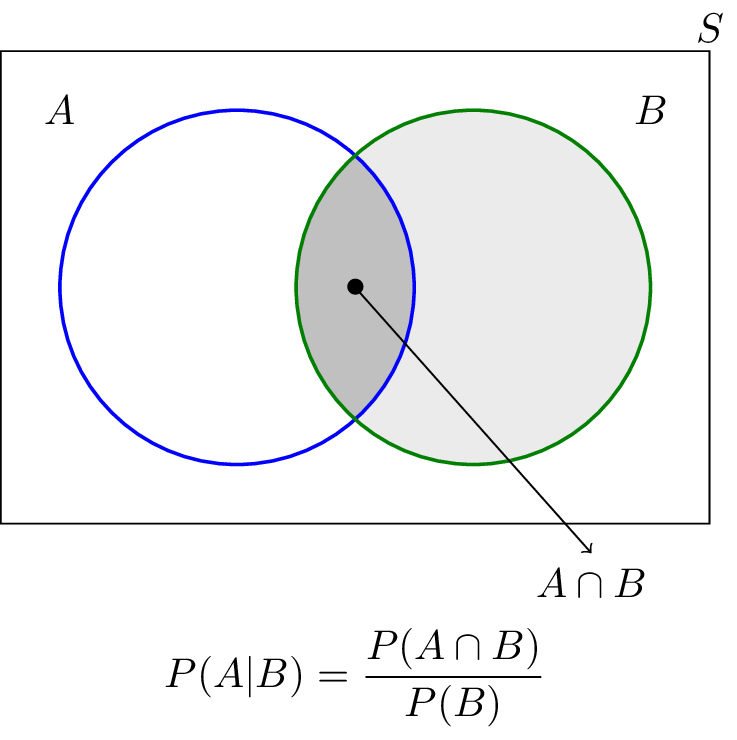
\includegraphics[width=0.5\columnwidth]{figures/uncert_fig_conditional_b.png}
\end{center}
\end{slide}

\begin{slide}
\slhead{Conditional Probability: Example}

We toss a die.\\
Someone tells you that the outcome is an even number.\\
What is the probability that the outcome is 6?
\begin{center}
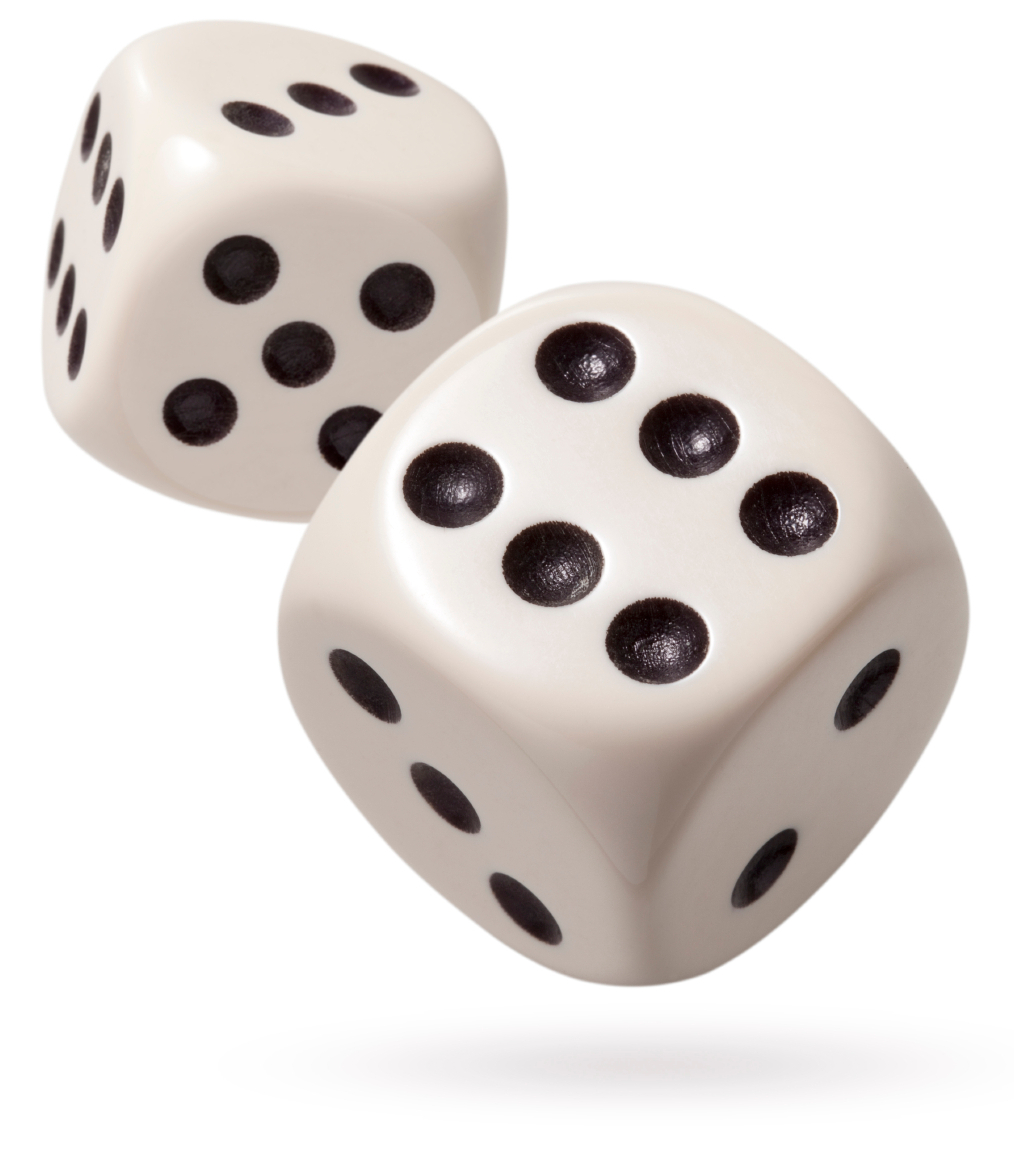
\includegraphics[width=0.4\columnwidth]{figures/uncert_fig_dice1.jpg}
\end{center}
\pause
1/3
\end{slide}


\begin{slide}
\slhead{Conditioning}
Possible values before evidence:
\begin{center}
\includegraphics[width=0.5\textwidth]{\figdir/worlds}
\end{center}
\pause
Observe $Color=orange$:
\begin{center}
\includegraphics[width=0.5\textwidth]{\figdir/worlds_orange}
\end{center}
\end{slide}


\begin{slide}
\slhead{Marginals}

If you have a joint probability distribution $P(X,Y)$ over some random variables $X,Y$,
the marginal distribution $P(X)$ can be computed by summing over all values of $Y$:

\begin{itemize}
\item $P(X) = \sum_Y P(X,Y)$
\end{itemize}

\end{slide}




\begin{slide}
\slhead{Exercise}
\begin{columns}
\begin{column}{6cm}
\begin{tabular}{|lll|l|}\hline
$Flu$ &  $Sneeze$ & $Snore$ & $\mu$\\
\hline
true & true & true & 0.064 \\
true & true & false & 0.096 \\
true & false & true & 0.016\\
true & false & false & 0.024 \\
false & true & true & 0.096 \\
false & true & false & 0.144 \\
false & false & true & 0.224 \\
false & false & false & 0.336 \\\hline
\end{tabular}
\end{column}

\begin{column}{6cm}
What is:
\begin{enumeratea}
\item $P(flu \land sneeze)$ % 0.16
\item $P(flu \land \neg sneeze)$ % 0.04
\item $P(flu)$ % 0.2
\item $P(sneeze\mid flu)$ % 0.8
\item $P(\neg flu  \land sneeze)$ % 0.24
\item $P(flu \mid sneeze)$ % 0.4
\item $P(sneeze\mid flu \land snore)$ % 0.064/(0.064+0.016) = 0.8
\item $P(flu\mid sneeze \land snore)$ % 0.064/(0.064+0.096) = 0.4
\end{enumeratea}
\end{column}
\end{columns}
\end{slide}


\begin{slide}
\slhead{Chain Rule}
%\begin{itemize}
%\item \textbf{Chain rule:}
\begin{eqnarray*}
\lefteqn{P(f_{1}\wedge f_{2}\wedge \ldots \wedge f_{n})}\\
&=&\pause
P(f_{n}|f_{1}\wedge \cdots \wedge f_{n-1}) \times \mbox{}\\
&&P(f_{1}\wedge \cdots
\wedge f_{n-1})\\
&=&\pause
P(f_{n}|f_{1}\wedge \cdots \wedge f_{n-1}) \times \mbox{}\\
&&P(f_{n-1}|f_{1}\wedge \cdots \wedge f_{n-2}) \times \mbox{}\\
&&P(f_{1}\wedge \cdots \wedge f_{n-2})\\
&=&
P(f_{n}|f_{1}\wedge \cdots \wedge f_{n-1}) \times \mbox{}\\
&&P(f_{n-1}|f_{1}\wedge \cdots \wedge f_{n-2})\\
&&\times{}\cdots \times
P(f_{3}|f_1 \wedge f_2)\times{}
P(f_{2}|f_1)\times{}
P(f_{1})
\\
&=& \prod_{i=1}^n P(f_i|f_{1}\wedge \cdots \wedge f_{i-1})
\end{eqnarray*}
%\end{itemize}
\end{slide}
\begin{slide}
\slhead{Bayes' theorem}
The chain rule and commutativity of conjunction ($h\wedge e$ is
equivalent to $e\wedge h$) gives us:
\begin{eqnarray*}
P(h\wedge e) & = & \pause P(h|e) \times P(e)\\
\pause
&=& P(e|h)\times P(h).
\end{eqnarray*}
\pause
If $P(e)\neq 0$,  divide the right hand sides by $P(e)$:
\[{P(h | e ) =
\pause \frac{P(e | h ) \times  P(h )}{P(e )}}.\]
This is \textbf{Bayes' theorem.}

\end{slide}
\begin{slide}
\slhead{Why is Bayes' theorem interesting?}
\begin{itemize}
\item Often you have causal knowledge:\\
$P(symptom~|~disease)$\\
%$P(light~is~off ~|~ status~of~switches~and~switch~positions)$\\
%$P(alarm ~|~ fire)$\\
%$P(image~looks~like {\includegraphics[height=14pt]{\figdir/car_tree}} ~|~ a~tree~is~in~front~of~a~car)$
\item and want to do evidential reasoning:\\
$P(disease~|~symptom)$\\
%$P(status~of~switches ~|~ light~is~off~and~switch~positions)$\\
%$P(fire~|~alarm)$.\\
%$P(a~tree~is~in~front~of~a~car~|~image~looks~like~{\includegraphics[height=14pt]{\figdir/car_tree}})$
%\item Bayes' theorem tells you how.
\end{itemize}
\end{slide}

\begin{slide}
\slhead{Exercise}
A cab was involved in a hit-and-run accident at night. Two cab
companies, the Green and the Blue, operate in the city. You are given:
\begin{itemize}
\item 85\% of the cabs in the city are Green and 15\% are Blue.
\item A witness identified the cab as Blue.
\item The witness reliability is 80\%.
\end{itemize}
What is the probability that the cab involved in the accident was
Blue?

\tiny{D. Kahneman, Thinking Fast and Slow, 2011, p. 166.}
\end{slide}

\begin{slide}
\slhead{Exercise: Solution}
$P(\text{cab is blue} | \text{witness says cab is blue}) =$ \\
~\\
$\frac{P(\text{witness says blue} | \text{cab is blue}) \times P(\text{cab is blue})}{P(\text{witness says blue})} =$ \\
~\\
$\frac{0.8 \times 0.15}{0.29} \approx $\\
~\\
$0.41$\\
~\\
(The normalizing constant ($P(\text{witness says blue})$) can be computed by marginalizing (summing over hypotheses): $0.8*0.15+0.2*0.85 = 0.29$.)
\end{slide}

%%%%%%%%%%%%%%%%%%%%%%%%%%%%%%%%%%%%%%%%%%%%%%%%%%%%%%%%%%%%%%%%%%%%%%%%%%%%%%%%

% SLIDES FROM LECT02:

%%%%%%%%%%%%%%%%%%%%%%%%%%%%%%%%%%%%%%%%%%%%%%%%%%%%%%%%%%%%%%%%%%%%%%%%%%%%%%%%



\begin{slide}
\slhead{Conditional independence}
Random variable $X$ is \textbf{independent} of random variable $Y$
\textbf{given}
random variable $Z$ if,
\[P(X|Y,Z) = P(X|Z)\]
\pause i.e. for all $x_i\in dom(X)$, $y_j\in dom(Y)$, $y_k\in dom(Y)$ and $z_m\in dom(Z)$,
\begin{eqnarray*}
\lefteqn{P(X=x_i|Y=y_j, Z=z_m)}\\
&=&P(X=x_i|Y=y_k, Z=z_m)\\
&=& P(X=x_i|Z=z_m).
\end{eqnarray*}
That is, knowledge of $Y$'s value doesn't affect the belief in
the value of $X$, given a value of $Z$.
%\begin{itemize}
%\item 
%\end{itemize}

\end{slide}
\begin{slide}
\slhead{Example domain (diagnostic assistant)}
%\vspace{1em}
\begin{center}
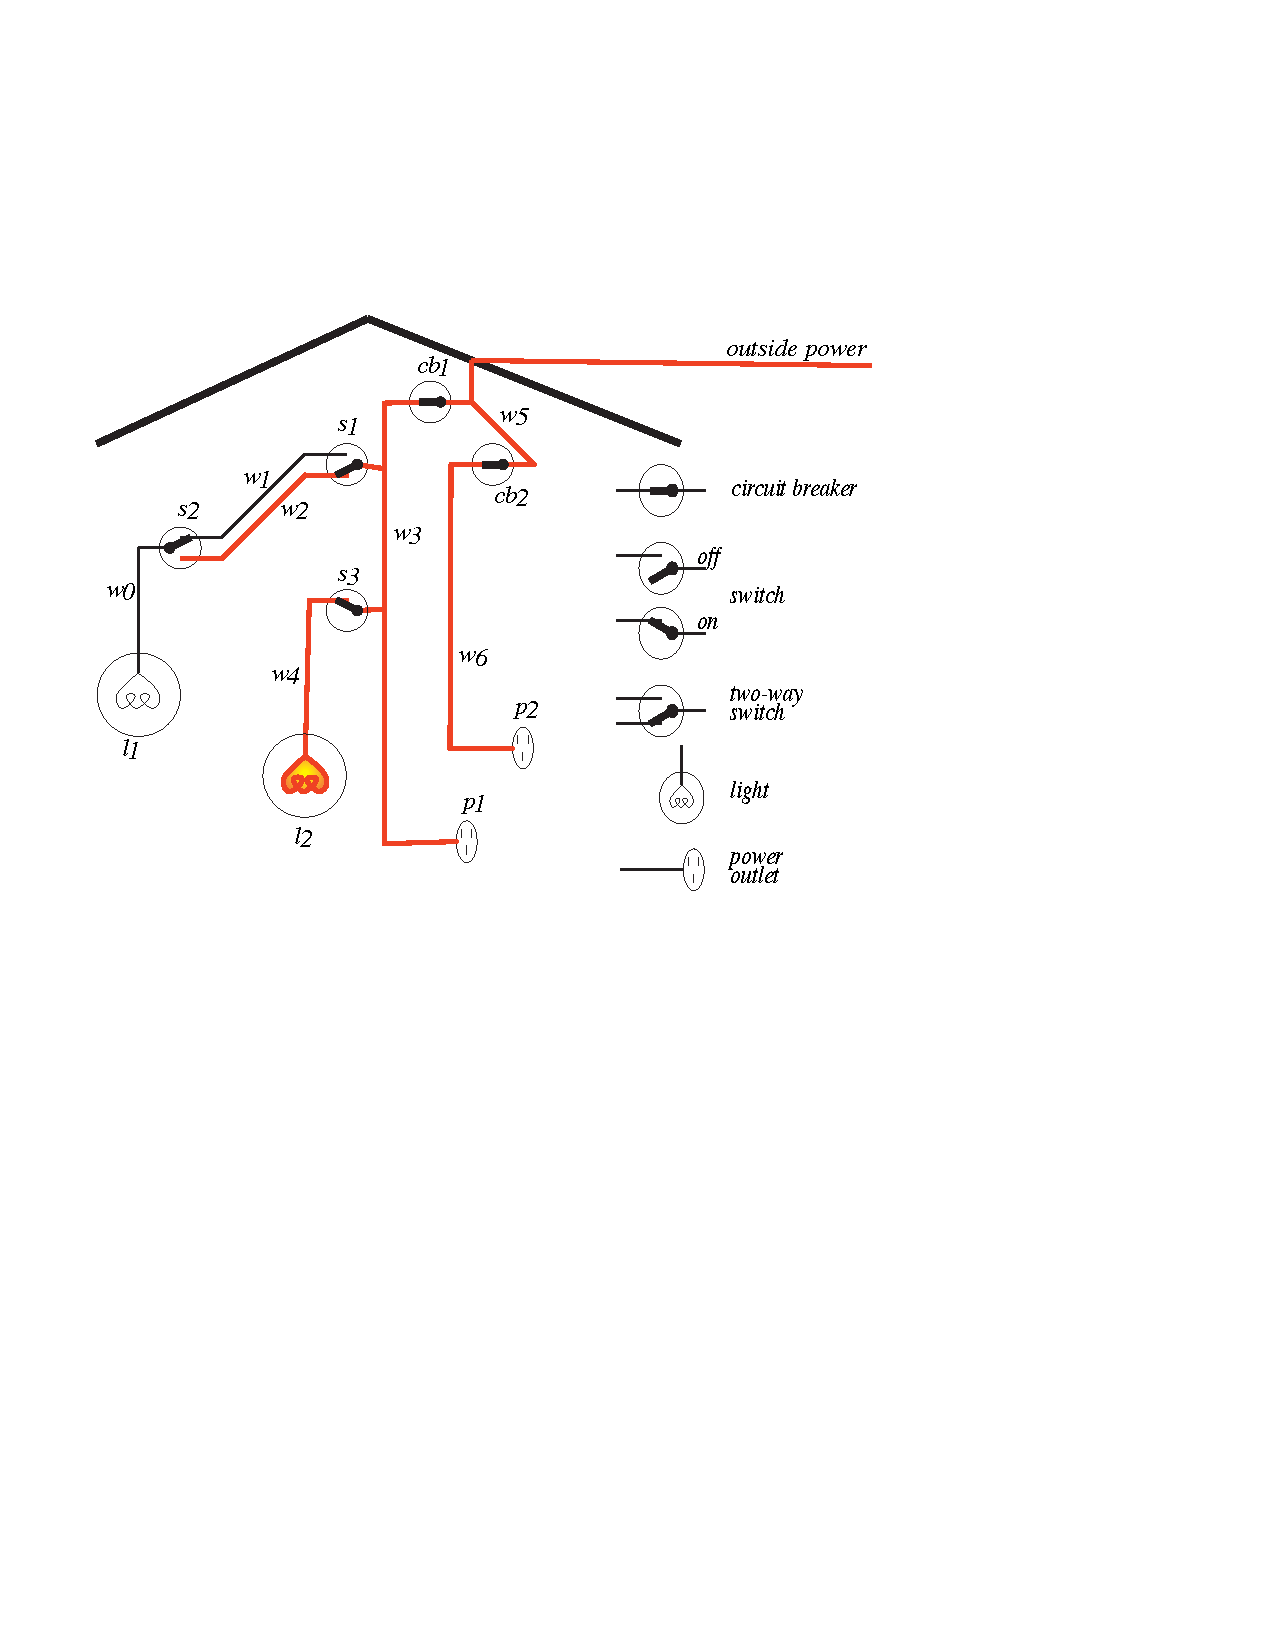
\includegraphics[width=0.85\textwidth]{\figdir/powerc}
\end{center}
%\vfill
\end{slide}
\begin{slide}
\slhead{Examples of conditional independence?}
\begin{itemize}
\item The identity of the queen of Canada is dependent or independent of whether
light $l1$ is lit given whether there is outside power?
\item Whether there is someone in a room is independent of whether a
light $l2$ is lit given what? %the position of switch $s3$.
\item Whether 
light $l1$ is lit is independent of the position of light switch $s2$
given what?% whether there is power in wire $w_0$.
\item Every other variable may be independent of whether 
light $l1$ is lit given \pause
whether there is power in wire $w_0$ and 
the status of light $l1$ (if it's $ok$, or if not, how it's broken).
\end{itemize}

\end{slide}
\begin{slide}
\slhead{Idea of belief networks}
\begin{minipage}[b]{0.5\textwidth}
%\item
\begin{itemize}
\item
 $l1$ is lit ($L1\_lit$) depends only on the status of the
light ($L1\_st$) and whether there is power in wire $w0$.
%Thus, $L1\_lit$ is independent of the other variables given $L1\_st$ and
%$W0$. 
\item In a belief network, $W0$ and $L1\_st$ are \textbf{parents} of
  $L1\_lit$.
\end{itemize}
\end{minipage}%
%\begin{center}
\includegraphics[width=0.5\textwidth]{\figdir/pow_bn_det}%
%\end{center}

\begin{itemize}
\item $W0$ depends only on \pause whether there is power in $w1$,
whether there is power in $w2$, the position of switch $s2$
($S2\_pos$), and the status of switch $s2$ ($S2\_st$).
\end{itemize}

\end{slide}

\begin{slide}
\slhead{Belief networks}
%Suppose $\{x_1,\dots,x_n\}$ are the variables of interest.
\begin{itemize}
\item Totally order the variables of interest: $X_1,\dots,X_n$
\item Theorem of probability theory (chain rule):\\
$
P(X_1,\ldots,X_n) =\prod_{i=1}^n P(X_i|X_1,\dots,X_{i-1})
$
\item  The \textbf{parents} $\parents{X_i}$ of $X_i$ are those predecessors of $X_i$ that
render $X_i$ independent of the other predecessors. That is, \pause 
$\parents{X_i} \subseteq X_1,\dots,X_{i-1}$ and
$P(X_i|\parents{X_i}) = P(X_i|X_1,\dots,X_{i-1})$
\item So
$P(X_1,\ldots,X_n) = \prod_{i=1}^n P(X_i|\parents{X_i})$
\item A \textbf{belief network} is a graph: the nodes are random
variables; there is an arc from the parents of each node into that
node.
\end{itemize}
\end{slide}

\begin{slide}
\slhead{Example: fire alarm belief network}
Variables:
\begin{itemize}
\item \alert{Fire}: there is a fire in the building
\item \alert{Tampering}: someone has been tampering with the fire alarm
\item \alert{Smoke}: what appears to be smoke is coming from
  an upstairs window
\item \alert{Alarm}: the fire alarm goes off
\item \alert{Leaving}: people are leaving the building \emph{en
    masse}.
\item \alert{Report}: a colleague says that people are leaving the
  building  \emph{en
    masse}. (A noisy sensor for leaving.)
\end{itemize}
\end{slide}


\begin{slide}
\slhead{Components of a belief network}
A belief network consists of:
\begin{itemize}
\item a directed acyclic graph with nodes
labeled with random variables
\item a domain for each random
variable 
\item a set of conditional probability tables for each variable given
its parents (including prior probabilities for nodes
with no parents).
\end{itemize}
\end{slide}


\begin{slide}
\slhead{Example belief network}
\begin{center}
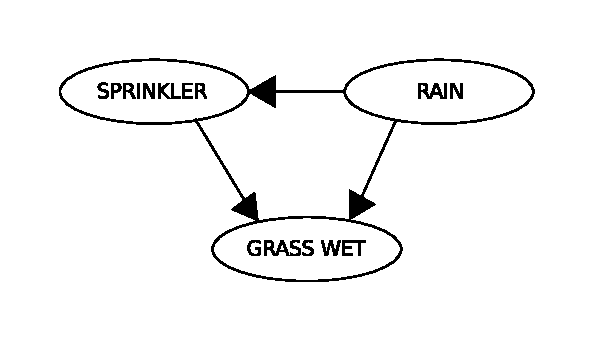
\includegraphics[width=0.6\textwidth]{figures/uncert_fig_bayes-net.pdf}
\end{center}
\end{slide}

\begin{slide}
\slhead{Components of a belief network}
A belief network consists of:
\begin{itemize}
\item a directed acyclic graph with nodes
labeled with random variables
\item a domain for each random
variable 
\item a set of conditional probability tables for each variable given
its parents (including prior probabilities for nodes
with no parents).
\end{itemize}
\end{slide}
\begin{slide}
\slhead{Example belief network}
\begin{center}
\includegraphics[width=\textwidth]{\figdir/power-bn}
\end{center}
\end{slide}



\begin{slide}
\slhead{Example belief network (continued)}
The belief network also specifies:
\begin{itemize}
\item The domain of the variables:\\
$W_0,\ldots,W_6$ have domain $\{live,dead\}$\\
$S_1\_pos$, $S_2\_pos$, and $S_3\_pos$ have  domain $\{up,down\}$\\
$S_1\_st$ has $\{ok,upside\_down,short,intermittent,broken\}$.
\item Conditional probabilities, such as:\\
$P(W_1=live|s_1\_pos=up \AND S_1\_st=ok \AND W_3=live)$\\
%$P(W_1=live|s_1\_pos=up \AND S_1\_st=ok \AND W_3=dead)$\\
%$P(W_1=live|s_1\_pos=up \AND S_1\_st=upside\_down \AND W_3=live$\\
%$P(S_1\_pos=up)$\\
%$P(S_1\_st=upside\_down)$
\end{itemize}
\end{slide}

\begin{slide}
\slhead{Belief network summary}
\begin{itemize}
\item A belief network is a directed acyclic graph (DAG).
\item Its nodes are random variables.
\item The \textbf{parents} of $X$ are those that $X$ directly depends on.
\item Acyclic by construction.
\item A representation of \textbf{dependence} and \textbf{independence}:
\begin{itemize}
\item $X$ is independent of its non-descendants given its parents.
\end{itemize}
\end{itemize}
\end{slide}

\begin{slide}
\slhead{Constructing belief networks}
%To represent a domain in a belief network, y
%You need to consider:
\begin{itemize}
\item What are the relevant variables?
\begin{itemize}
\item Observed?
\item Query variables?
\item Variables that make the model simpler?
\end{itemize}
\item What values should these variables take?
\item What is the relationship between them?
% This should be expressed
%in terms of a directed graph, representing how each variable is
%generated from its predecessors.
\item How does the value of each variable depend on its parents?
% This is expressed in terms of the
%conditional probabilities.
\end{itemize}
\end{slide}

\begin{slide}
\slhead{Using belief networks}
%The example power network can be used in a number of ways:
An example of how the power network can be used:
\begin{itemize}
%\item Conditioning on the status of the switches and circuit
%breakers, whether there is outside power and the
%position of the switches, you can simulate the lighting.
%\item Given values of the outside power and the position of the
%switches, you can determine how likely 
%it is that any light is lit.
\item Given values for:
  \begin{itemize}
    \item switches,
    \item outside power,
    \item whether the lights are lit,
  \end{itemize}
\item you can determine the posterior probability that each switch or circuit breaker is ok or not.
%\item Given some observations, you can use the network to reason
%backwards to determine the most 
%likely position of switches.
%\item Given some switch positions and some outputs and some
%intermediate values, you can determine the probability of any other
%variable in the network.
\end{itemize}
\end{slide}

\begin{slide}
\slhead{Using belief networks}

This is called \textbf{inference}.\\
~\\
~\\


\begin{center}
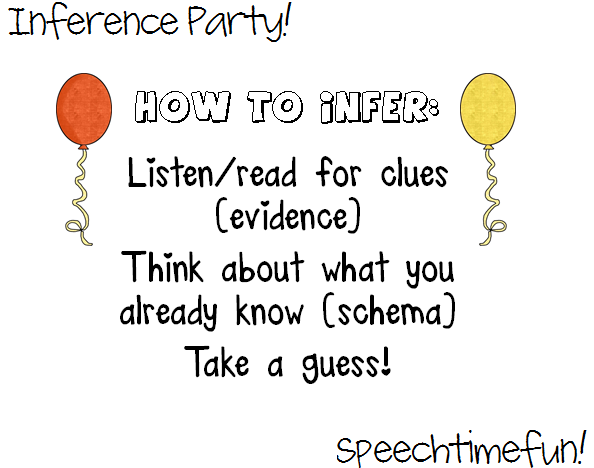
\includegraphics[width=0.6\textwidth]{figures/uncert_fig_inference2.png}
\end{center}

\end{slide}

% \begin{slide}
% \slhead{Inferring conditional probabilities (I)}
% If observation $e$ doesn't involve $X$ or a descendent of $X$:
% \begin{eqnarray*}
% \lefteqn{P(X|e) }\\
% &=& \sum_{v \in dom(\parents{X})} P(X \wedge \parents{X}=v|e)\\
% &=& \sum_{v \in dom(\parents{X})} P(X | \parents{X}=v \wedge
% e)P(\parents{X}=v|e)\\
% &=& \sum_{v \in dom(\parents{X})} P(X | \parents{X}=v)P(\parents{X}=v|e)
% \end{eqnarray*}

% \end{slide}

% \begin{slide}
% \slhead{Inferring conditional probabilities (II)}
% If you observe $Y=y \wedge e$ where $Y$ is a descendent of $X$:
% \begin{eqnarray*}
% P(X|Y=y \wedge e) &=& 
% \frac{P(Y=y|X \wedge e) P(X|e)}{P(Y=y|e)}
% \end{eqnarray*}

% \end{slide}


%%%%%%%%%%%%%%%%%%%%%%%%%%%%%%%%%%%%%%%%%%%%%%%%%%%%%%%%%%%%%%%%%%%%%%%%%%%%%%%%

% SLIDES FROM LECT03:

%%%%%%%%%%%%%%%%%%%%%%%%%%%%%%%%%%%%%%%%%%%%%%%%%%%%%%%%%%%%%%%%%%%%%%%%%%%%%%%%


\begin{slide}
\slhead{Understanding independence: example}
\begin{center}
\includegraphics[width=0.9\textwidth]{\figdir/indep-bn}
\end{center}


\end{slide}

\begin{slide}
\slhead{Understanding independence: questions}
\begin{itemize}
\item On which given probabilities does \textbf{$P(N)$} depend?
\item If you were to observe a value for \textbf{$B$,} which variables'
probabilities will change?
\item If you were to observe a value for \textbf{$N$,} which variables'
probabilities will change?
\item Suppose you had observed a value for $M$; if you were to then observe a value for \textbf{$N$,} which variables'
probabilities will change?
\item Suppose you had observed $B$ and $Q$; which variables'
probabilities will change when you observe \textbf{$N$?}
\end{itemize}


\end{slide}


\begin{slide}
\slhead{What variables are affected by observing?}
\begin{itemize}
\item If you observe variable $\overline{Y}$, the variables whose
posterior probability is different from their prior are:
\begin{itemize}
\item The ancestors of $\overline{Y}$ and
\item their descendants.
\end{itemize}
\item Intuitively (if you have a causal belief network):
\begin{itemize}
\item You do \textbf{abduction} to possible causes and
\item \textbf{prediction} from the causes.
\end{itemize}
\end{itemize}
\end{slide}

\begin{slide}
\slhead{Common descendants}
\begin{tabular}{lr}
\includegraphics{\figdir/common-desc}&
\begin{minipage}[b]{0.45\textwidth}
\begin{itemize}
\item $tampering$ and $fire$ are independent
\item $tampering$ and $fire$ are dependent given $alarm$
\item Intuitively, $tampering$ can \textbf{explain away} $fire$
\end{itemize}

\end{minipage}
\end{tabular}

\end{slide}

\begin{slide}
\slhead{Common ancestors}
\begin{tabular}{lr}
\includegraphics{\figdir/common-anc}&
\begin{minipage}[b]{0.45\textwidth}
\begin{itemize}
\item $alarm$ and $smoke$ are dependent
\item $alarm$ and $smoke$ are independent given $fire$
\item Intuitively, $fire$ can \textbf{explain} $alarm$ and $smoke$;
learning one can affect the other by changing your belief in $fire$.
\end{itemize}

\end{minipage}
\end{tabular}

\end{slide}
\begin{slide}
\slhead{Chain}
\begin{tabular}{lr}
\includegraphics{\figdir/chain}&
\begin{minipage}[b]{0.45\textwidth}
\begin{itemize}
\item $alarm$ and $report$ are dependent
\item $alarm$ and $report$ are independent given $leaving$
\item Intuitively, the only way that the $alarm$ affects $report$ is
by affecting $leaving$.
\end{itemize}

\end{minipage}
\end{tabular}

\end{slide}

%\begin{slide}
%\slhead{Pruning Irrelevant Variables}
%Suppose you want to compute $P(X|e_1\dots e_k)$:
%\begin{itemize}
%\item Prune any variables that have no observed or queried descendents.
%\item Connect the parents of any observed variable.
%\item Remove arc directions.
%\item Remove observed variables.
%\item Remove any variables not connected to $X$ in the resulting
%  (undirected) graph.
%\end{itemize}

%\end{slide}

\if 0
\begin{slide}
\slhead{d-separation}
\begin{itemize}
\item
$\overline{X}$ is \textbf{d-separated} from $\overline{Y}$ given $\overline{Z}$
if there is no path from an element of $\overline{X}$ to an element of
$\overline{Y}$,
where:
\begin{itemize}
\item If there are paths $A \rightarrow B$ and $B \rightarrow C$ such
that $B \not \in \overline{Z}$, there is a path $A\rightarrow C$.
\item If there are paths $B\rightarrow A$ and $B \rightarrow C$ such
that $B \not \in \overline{Z}$, there is a path $A \rightarrow C$.
\item If there are paths $A \rightarrow B$ and $C \rightarrow B$ such
that $B \in \overline{Z}$, there is a path $A \rightarrow C$.
\end{itemize}
\item $\overline{X}$ is independent $\overline{Y}$ given
$\overline{Z}$ for some conditional probabilities iff $\overline{X}$ is d-separated from $\overline{Y}$
given $\overline{Z}$
\end{itemize}

\end{slide}
\fi

%%%%%%%%%%%%%%%%%%%%%%%%%%%%%%%%%%%%%%%%%%%%%%%%%%%%%%%%%%%%%%%%%%%%%%%%%%%%%%%%

% SLIDES FROM LECT04:

%%%%%%%%%%%%%%%%%%%%%%%%%%%%%%%%%%%%%%%%%%%%%%%%%%%%%%%%%%%%%%%%%%%%%%%%%%%%%%%%



\newcommand{\smeq}{\,{=}\,}

\begin{slide}
\slhead{Belief network inference}
%Four main approaches to determine posterior distributions in belief networks:
\begin{itemize}
\item Variable Elimination: exploit the structure of the network to eliminate (sum out) the
non-observed, non-query variables one at a time.
\item Search-based approaches: enumerate some of the
possible assignments, and estimate posterior probabilities.
\item Stochastic simulation: generate random assignments according to the probability distributions.
\item Variational methods: find the closest tractable
  distribution to the (posterior) distribution.
\end{itemize}
\end{slide}

% \begin{slide}
% \slhead{Summing out a variable: intuition}
% Suppose $B$ is Boolean ($B=true$ is $b$ and $B=false$ is $\neg b$)
% \begin{tabular}{rl}
% \includegraphics[width=20mm]{\figdir/abcbn-new} &
% \begin{tabular}[b]{l}
% $\begin{array}[b]{rcl}
% \lefteqn{P(C|A)}\\
%  &=& P(C\AND b | A) + P(C\AND \neg b | A)\\
% &=& P(C|b \AND A) P(b|A) + P(C|\neg b \AND A) P(\neg b|A)\\
% &=& P(C|b) P(b|A) + P(C|\neg b) P(\neg b|A)\\
% &=& \sum_B P(C|B) P(B|A)\\
% \end{array}$
% \\
% We can compute the probability of some of
% the \\variables by summing out
% the other variables.
% \end{tabular}

% \end{tabular}
% \end{slide}

\begin{slide}
\slhead{Factors}
Function from
a set of random variables to a number. $f(X_1,\ldots,X_j)$.

Some or all of the variables of a factor can be assigned:
\begin{itemize}
\item
$f(X_1{\smeq}v_1,X_2,\ldots,X_j)$,
is a factor on
$X_2,\ldots,X_j$.
\item 
$f(X_1{\smeq}v_1,X_2{\smeq}v_2,\ldots,X_j{\smeq}v_j)$  is a number that is the value of $f$ when each
$X_i$ has value $v_i$. 
\end{itemize}
%The former is also written as $f(X_1,X_2,\ldots,X_j)_{X_1{\smeq}v_1}$, etc.
\end{slide}

\begin{slide}
\slhead{Example factors}
$r(X,Y,Z)$:\begin{tabular}{|lll|r|}
\hline
$X$ & $Y$ &$Z$ & val\\\hline
t & t & t & 0.1\\
t & t & f & 0.9\\
t & f & t & 0.2\\
t & f & f & 0.8\\
f & t & t & 0.4\\
f & t & f & 0.6\\
f & f & t & 0.3\\
f & f & f & 0.7\\\hline
\end{tabular}
\begin{tabular}{r}
$r(X{=}t,Y,Z)$:\begin{tabular}{|ll|r|}
\hline
$Y$ &$Z$ & val\\\hline
t & t & 0.1\\
t & f & \uncover<2>{0.9}\\
f & t &  \uncover<2>{0.2}\\
f & f &  \uncover<2>{0.8}\\
\hline
\end{tabular}\\*[1.75cm]
\pause
$r(X{=}t,Y,Z{=}f)$:\pause\begin{tabular}{|l|r|}
\hline
$Y$ & val\\\hline
t &  \uncover<4>{0.9}\\
f &  \uncover<4>{0.8}\\\hline
\end{tabular}\\
$r(X{=}t,Y{=}f,Z{=}f)=\ \uncover<4>{0.8}$
\end{tabular}


\end{slide}


\begin{slide}
\slhead{Multiplying factors}
The  \textbf{product} of factor $f_1(\overline{X},\overline{Y})$ and
$f_2(\overline{Y},\overline{Z})$, where $\overline{Y}$ are the
variables in common, is the factor $(f_1 \times
f_2)(\overline{X},\overline{Y},\overline{Z})$ defined by:
\begin{eqnarray*}
%\lefteqn{
(f_1 \times f_2)(\overline{X},\overline{Y},\overline{Z}) %}\\
&=&
f_1(\overline{X},\overline{Y}) f_2(\overline{Y},\overline{Z}).
\end{eqnarray*}

\end{slide}

\begin{slide}
\slhead{Multiplying factors example}
\begin{center}
{\renewcommand{\arraystretch}{0.9}
\begin{tabular}{r}
$f_1$: \begin{tabular}{|ll|r|}
\hline
$A$ &$B$ & val\\\hline
t & t & 0.1\\
t & f & 0.9\\
f & t & 0.2\\
f & f & 0.8\\
\hline
\end{tabular}\\\mbox{}\\
$f_2$: \begin{tabular}{|ll|r|}
\hline
$B$ &$C$ & val\\\hline
t & t & 0.3\\
t & f & 0.7\\
f & t & 0.6\\
f & f & 0.4\\
\hline
\end{tabular}\\
\end{tabular}
\hspace{1cm}
$f_1 \times f_2$: \begin{tabular}{|lll|r|}
\hline
$A$ & $B$ &$C$ & val\\\hline
t & t & t & 0.03\\
t & t & f &  \uncover<2>{0.07}\\
t & f & t &  \uncover<2>{0.54}\\
t & f & f &  \uncover<2>{0.36}\\
f & t & t &  \uncover<2>{0.06}\\
f & t & f &  \uncover<2>{0.14}\\
f & f & t &  \uncover<2>{0.48}\\
f & f & f &  \uncover<2>{0.32}\\\hline
\end{tabular}
}
\end{center}
\end{slide}

\begin{slide}
\slhead{Summing out variables}
We can
\textbf{sum out} a variable, say $X_1$ with domain
$\{v_1,\ldots,v_k\}$, from factor $f(X_1,\ldots,X_j)$,
resulting in a factor on $X_2,\ldots,X_j$
defined by:
\begin{eqnarray*}
\lefteqn{(\sum_{X_1} f)(X_2,\ldots,X_j)}\\
& =& f(X_1{\smeq}v_1,\ldots,X_j)+ \cdots + 
f(X_1{\smeq}v_k,\ldots,X_j)
\end{eqnarray*}


\end{slide}
\begin{slide}
\slhead{Summing out a variable example}
\begin{center}

$f_3$: \begin{tabular}{|lll|r|}
\hline
$A$ & $B$ &$C$ & val\\\hline
t & t & t & 0.03\\
t & t & f & 0.07\\
t & f & t & 0.54\\
t & f & f & 0.36\\
f & t & t & 0.06\\
f & t & f & 0.14\\
f & f & t & 0.48\\
f & f & f & 0.32\\\hline
\end{tabular}
\hspace{1cm}
$\sum_B f_3$: \begin{tabular}{|ll|r|}
\hline
$A$ & $C$ & val\\\hline
t & t & 0.57\\
t & f &  \uncover<2>{0.43}\\
f & t &  \uncover<2>{0.54}\\
f & f &  \uncover<2>{0.46}\\
\hline
\end{tabular}
\end{center}
\end{slide}

\begin{slide}
\slhead{Exercise}
Given factors:

s: \begin{tabular}{|l|r|}
\hline
$A$ & val\\\hline
t &  0.75\\
f &  0.25\\\hline
\end{tabular}
~~~~
t: \begin{tabular}{|ll|r|}
\hline
$A$ &$B$ & val\\\hline
t & t & 0.6\\
t & f & 0.4\\
f & t & 0.2\\
f & f & 0.8\\
\hline
\end{tabular}
~~~~~
o: \begin{tabular}{|l|r|}
\hline
$A$ & val\\\hline
t &  0.3\\
f &  0.1\\\hline
\end{tabular}

What is?
\begin{enumeratea}
\item $s \times t$
\item $\sum_A s \times t$
\item $\sum_B s \times t$
\item  $s \times t \times o$
\item  $\sum_A s \times t \times o$
\item  $\sum_b s \times t \times o$
\end{enumeratea}
\end{slide}

\begin{slide}
\slhead{Evidence}
If we want to compute the posterior probability of $Z$ given evidence
$Y_1{\smeq}v_1\AND\ldots\AND Y_j{\smeq}v_j$:
\begin{eqnarray*}
\lefteqn{P(Z|Y_1{\smeq}v_1,\ldots,Y_j{\smeq}v_j)}\\
  &=&\pause \frac{ P(Z,Y_1{\smeq}v_1,\ldots,Y_j{\smeq}v_j)}{P(Y_1{\smeq}v_1,\ldots,Y_j{\smeq}v_j)} \\
  &=&\pause \frac{ P(Z,Y_1{\smeq}v_1,\ldots,Y_j{\smeq}v_j)}{\sum_{Z} P(Z,Y_1{\smeq}v_1,\ldots,Y_j{\smeq}v_j).}
\end{eqnarray*}
So the computation reduces to the probability of
$P(Z,Y_1{\smeq}v_1,\ldots,Y_j{\smeq}v_j)$.

We normalize at the end.
\end{slide}

\end{document}
